\section{Модель термической деполимеризации ПММА}

В данном разделе описывается моделирование локального распределения молекулярной массы ПММА при экспонировании резиста ``в кадр'' в процессе СЭЛТР. Начальные значения среднечисловой ($\Mn$) и средневесовой ($\Mw$) молекулярной массы ПММА приняты равными соответственно 271374 и \linebreak 669184, что соответствует резисту PMMA 950K A2 от компании ``Allresist'', использовавшемуся в данной работе. Величина тока при экспонировании принята равной 5 нА, энергия электронного пучка -- 20 кэВ, размеры экспонируемой области -- \linebreak 2.4$\times$1.9 мм$\pp$, толщина слоя ПММА -- 500 нм, расстояние между линиями -- 3 мкм, время экспонирования -- 100 с, температура образца -- 130~$^\circ$C. Данные значения согласуются со значениями соответствующих параметров в ранее проводившихся экспериментах по изучению метода СЭЛТР~\cite{Bruk_2016_mee}. Полное число линий в экспериментах при экспонировании ``в кадр'' составляло 625, однако для уменьшения требуемого машинного времени моделирование проводилось для участка одной линии длиной 100~нм с применением периодических граничных условий. На основе промоделированного распределения актов электрон-электронного взаимодействия в слое ПММА и вероятности разрыва (0.08 для 130~$^\circ$C) рассчитывалось распределение разрывов молекул ПММА. $x-$ и $z-$координаты актов разрыва собирались в двумерные гистограммы с размером бина 50 нм по обеим осям. Примеры таких гистограмм, полученных для различных значений времени экспонирования приведены на рисунке~\ref{fig:scission_hist}.

\begin{figure}[t]
	\begin{center}
		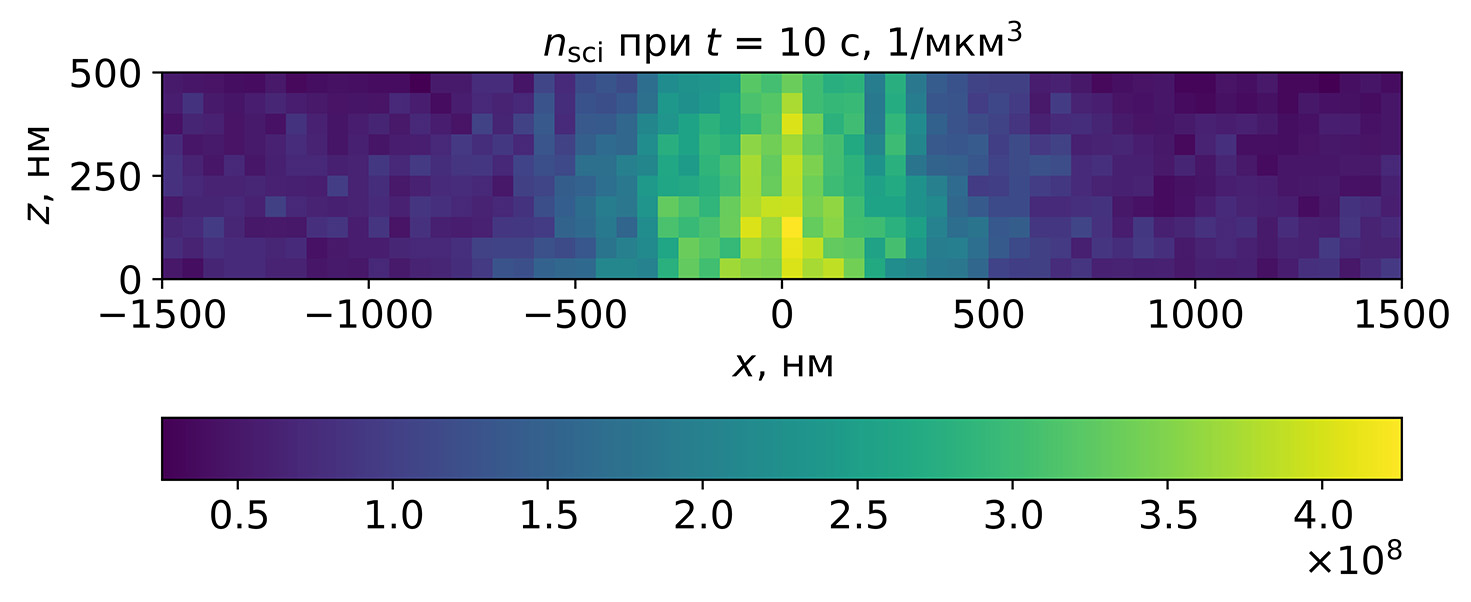
\includegraphics[width=0.8\linewidth]{MW/sci_conc_10s_straight_200} \\
		\vspace{-3.7em} \text{\hspace{-26em} a)} \vspace{2.7em} \\
		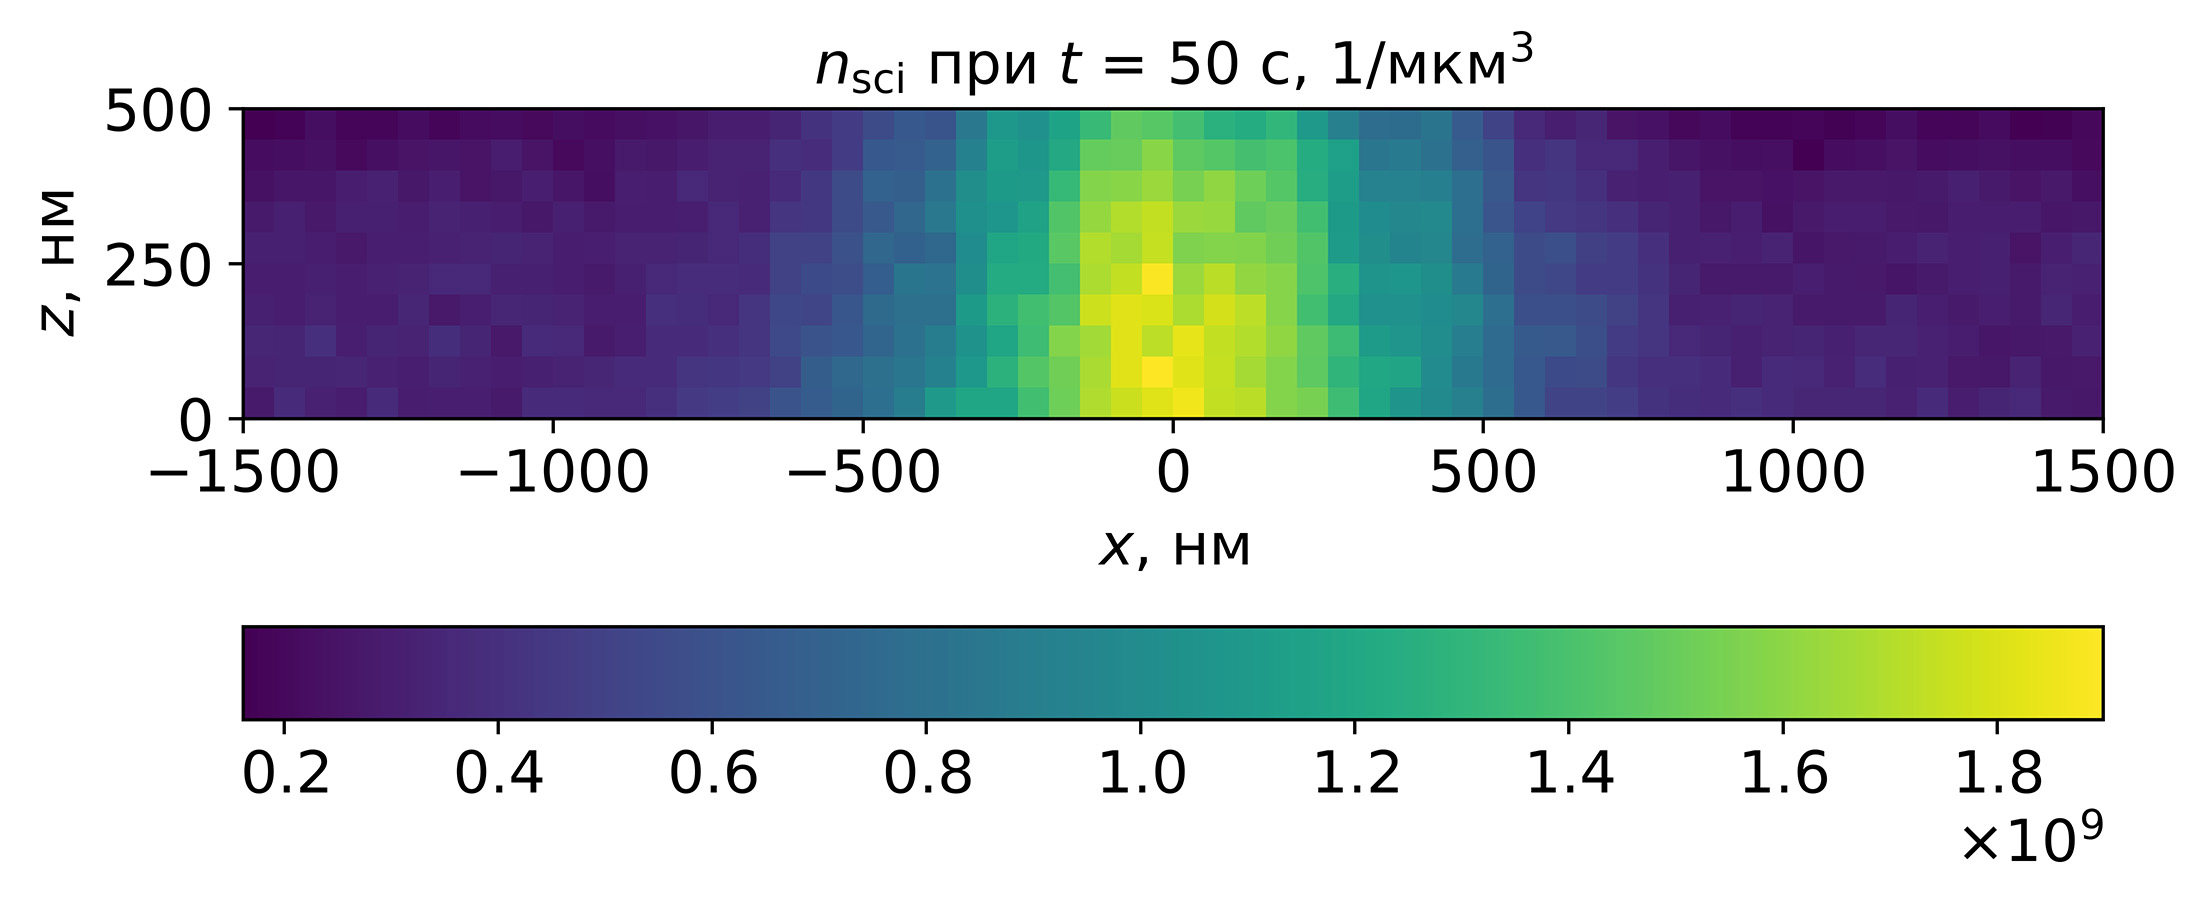
\includegraphics[width=0.8\linewidth]{MW/sci_conc_50s_straight_200} \\
		\vspace{-3.7em} \text{\hspace{-26em} б)} \vspace{3.7em} \\
	\end{center}
	\vspace{-2.5em}
	\caption{Концентрация разрывов в слое ПММА при различных значениях времени экспонирования при температуре 130~$^\circ$C.}
	\label{fig:scission_hist}
\end{figure}

Для нахождения распределения локальной молекулярной массы резиста была использована модель, описанная в разделе~\ref{sec:depolymerization}. Было использовано предположение о том, что распределение молекулярной массы резиста PMMA 950K A2, использовавшегося в экспериментах, описывается функцией распределения Шульца-Цимма со значениями среднечисловой и средневесовой молекулярной массы, равными 271374 и 669184 соответственно:
\begin{equation} \label{eq:Schulz-Zimm_distribution}
	P_n = C_0 n^z \exp (-n/y).
\end{equation}
Начальные значения параметров этого распределения ($z_0$ и $y_0$) были найдены на основе формул \ref{eq:Schulz-Zimm_1} и \ref{eq:Schulz-Zimm_2}:
\begin{equation}
	\begin{aligned}
		PD & \equiv \frac{\Mw}{\Mn} = \frac{669184}{271374} \cong 2.47, \\
		z_0 & = (2-PD)/(PD-1) \cong -0.32, \\
		y_0 & = x_0/(z_0+1) \cong 3989.58.
	\end{aligned}
\end{equation}
Также, согласно результатам работы~\cite{Mita_PMMA_zip_lengths_T}, средняя длина цепи деполимеризации при 130~$^\circ$C была принята равной 500. После задания всех параметров система дифференциальных уравнений~\ref{eq:scary_system} решалась численно методом Рунге-Кутты 4 порядка с переходом на схему предиктор-корректор начиная с четвертого шага (рисунок~\ref{fig:SZ_M1_y_tau}). Диапазон значений переменной $\tau$ составлял от 0 до 400 с шагом 0.01.

\begin{figure}[t]
	\begin{minipage}{0.48\textwidth}
			\hspace{-0.5em} 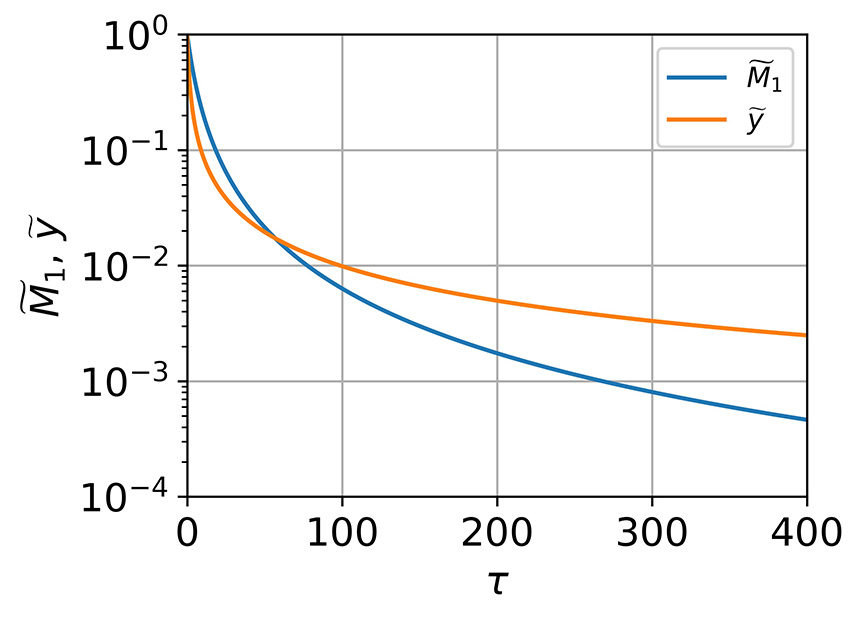
\includegraphics[width=\linewidth]{MW/SZ_M1_y_14_200} \\
			\vspace{-12.5ex} \\ \text{\hspace{3.8em} a}) \\ \vspace{12.5ex}
		\end{minipage}
	\begin{minipage}{0.48\textwidth}
			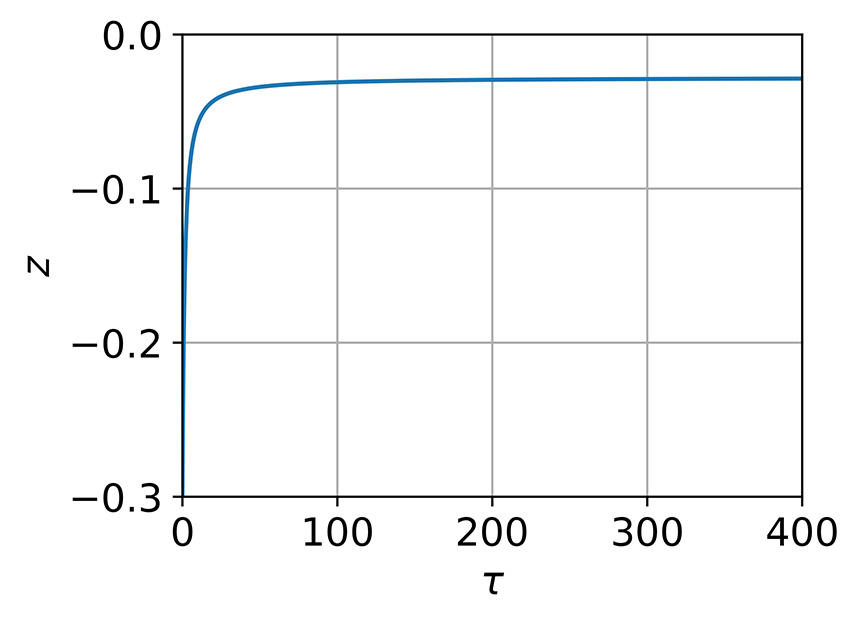
\includegraphics[width=\linewidth]{MW/SZ_z_14_200} \\
			\vspace{-12.5ex} \\ \text{\hspace{4em} б}) \\ \vspace{12.5ex}
		\end{minipage}
	\vspace{-3.5em}
	\caption{Зависимости параметров распределения Шульца-Цимма от безразмерной временной переменной $\tau$, полученные для резиста PMMA 950K A2, использовавшегося в данной работе.}
	\label{fig:SZ_M1_y_tau}
\end{figure}

Зависимость параметров распределения молекулярной массы резиста от безразмерной переменной $\tau$ далее пересчитывалась в зависимость от времени ($t$) на основе формулы~\ref{eq:dim_less_MW}:
\begin{equation} \label{eq:tau_y0_ks_t}
	\tau = y_0 k_\mathrm{s} t.
\end{equation}
Входящая в это выражение величина $k_\mathrm{s}$, выражающая количество разрывов молекул резиста за 1 секунду, приходящееся на 1 мономер, определялась из концентрации разрывов в каждой ячейке вышеописанных гистограмм следующим образом. Изначально была создана двумерная гистограмма с размерами, аналогичными размерам гистограмм, содержащих концентрацию разрывов, в каждую ячейку которой (условно с индексами $i$ и $j$) в качестве начального значения величины $\tau$ было записано число 0. Далее для каждой секунды экспонирования вычислялось число разрывов, относившихся к этой ячейке ($N_\mathrm{sci}^\mathrm{1c}[i,j]$). После этого прибавка к величине $\tau$ в данной ячейке, соответствующей 1 секунде экспонирования, определялась согласно формуле~\ref{eq:tau_y0_ks_t}:
\begin{equation}
	\Delta \tau_\mathrm{1c} [i,j] = 3989.58 \cdot \frac{N_\mathrm{sci}^\mathrm{1c}[i,j]}{1789618} \cdot 1с,
\end{equation}
где 1789618 -- число мономеров ПММА, соответствующее ячейке гистограммы размером 50$\times$100$\times$50 нм$\ppp$, рассчитанное на основе плотности ПММА и молярной массы ММА (1.19~г/см$\ppp$ и 100 г/моль соответственно). Величина $\Delta \tau_\mathrm{1c} [i,j]$ добавлялась к текущему значению $\tau$ для этой ячейке, что позволяло в каждый момент времени определить параметры распределения Шульца-Цимма для резиста в данной ячейке. Это позволило промоделировать локальные значение параметров $y$ и $z$ функции распределения молекулярной массы резиста и вычислить локальные значения среднечисловой и средневесовой молекулярной массы резиста в различные моменты времени по формулам
\begin{equation}
	\begin{aligned}
	M_\mathrm{n} [i,j] (t) & = y[i,j] (t) (z [i,j] (t) + 1), \\
	M_\mathrm{w} [i,j] (t) & = M_\mathrm{n} [i,j] (t) \cdot \frac{z[i,j] (t) + 2}{z[i,j] (t) + 1},
	\end{aligned}
\end{equation}
где 100 -- молярная масса ММА (в г/моль).

Промоделированные таким образом пространственные распределения локальной среднечисловой молекулярной массы ПММА для двух различных значений времени экспонирования приведены на рисунке~\ref{fig:Mn_hist}.

\begin{figure}[h]
	\begin{center}
		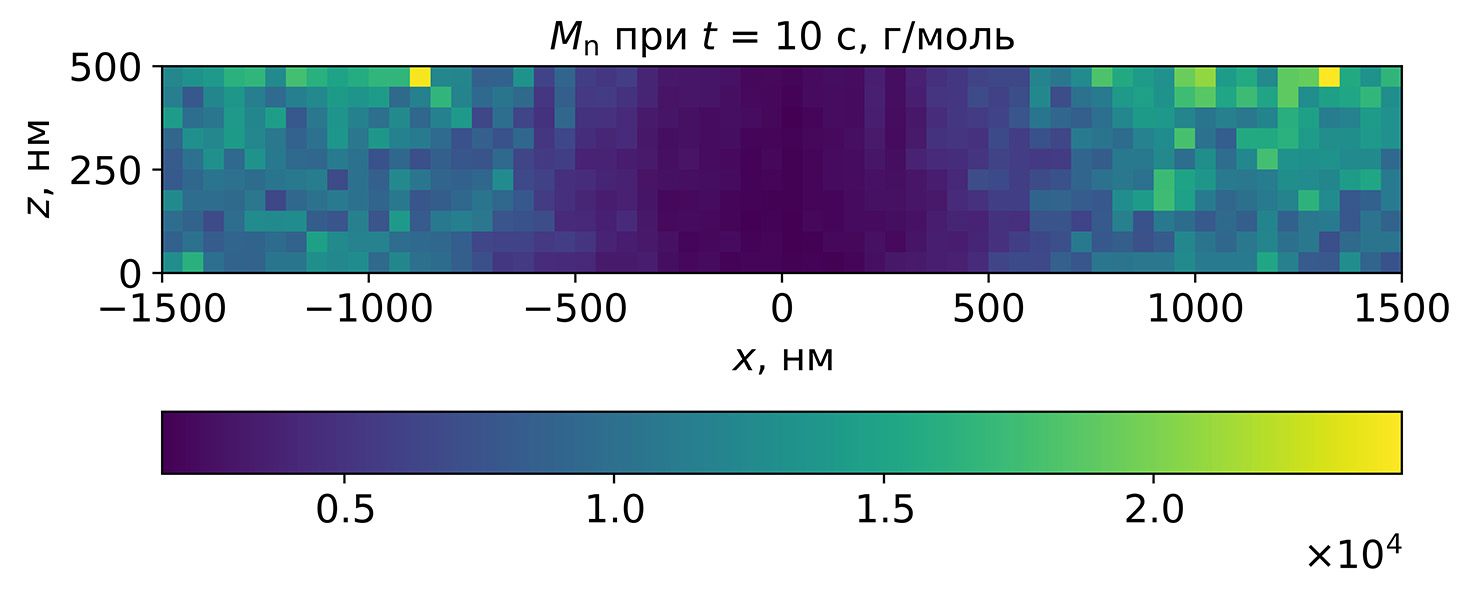
\includegraphics[width=0.8\linewidth]{MW/Mn_hist_10s_straight_200} \\
		\vspace{-3.7em} \text{\hspace{-26em} a)} \vspace{2.7em} \\
		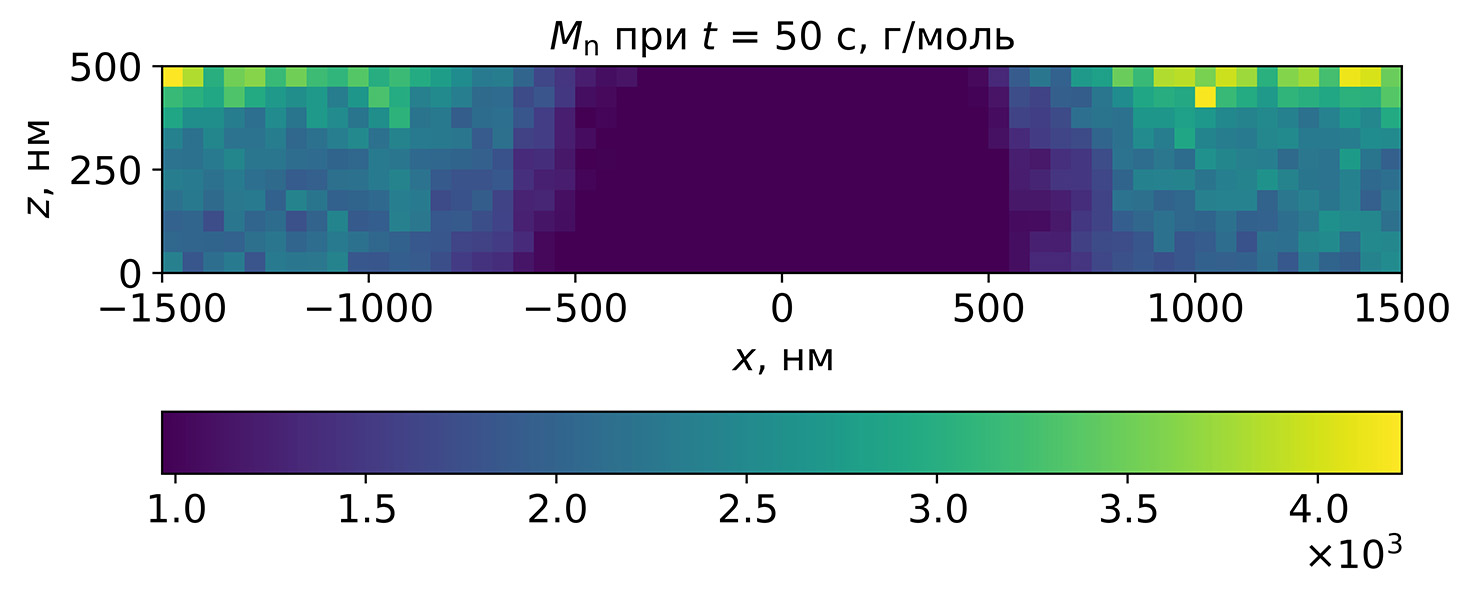
\includegraphics[width=0.8\linewidth]{MW/Mn_hist_50s_straight_200} \\
		\vspace{-3.7em} \text{\hspace{-26em} б)} \vspace{3.7em} \\
	\end{center}
	\vspace{-2.5em}
	\caption{Промоделированные распределения локальной среднечисловой молекулярной массы PMMA 950К A2 в различные моменты времени экспонирования при температуре 130~$^\circ$C. Экспонирование производилось ``в кадр'' с размерами 2.4$\times$1.9 мм$\pp$, число линий в кадре составляло 625, расстояние между линиями -- 3 мкм. Энергия электронного пучка равна 20 кэВ, ток экспонирования -- 5 нА.}
	\label{fig:Mn_hist}
\end{figure}
